\documentclass[12pt]{report}
\usepackage[margin=1in]{geometry}
\usepackage[english]{babel} 
\usepackage{amsmath,amsfonts,amsthm}
\usepackage{fancyhdr}
\usepackage{enumitem}
\usepackage{indentfirst}
   \usepackage{float}
      \usepackage{graphicx}

\pagestyle{fancy}
\fancyhf{}
\rhead{Eli Schmitter}
\lhead{HW6}
\rfoot{\thepage}

\begin{document}
\section*{6.3}
\subsection*{2}
 $$H_0:p>.60, H_1:p\leq.60$$\\
 $$\hat{p}=\frac{281}{444}=.633,p_0=.6$$
 \begin{align*}
 Z&=\frac{\hat{p}-p_0}{\sqrt{p_0(1-p_0)/n}}\\
  &=\frac{.633-.6}{\sqrt{.6(1-.6)/444}}\\
  &=1.42\\
  &\Rightarrow\\
 P&=.9222
 \end{align*}
 There for one could conclude that more than 60% of HIV-positive smokers aremale?.
\subsection*{4}
$$H_0:p>\geq.50,H_1<50$$
 $$\hat{p}=\frac{49}{73}=.671,p_0=.6$$
 \begin{align*}
 Z&=\frac{\hat{p}-p_0}{\sqrt{p_0(1-p_0)/n}}\\
  &=\frac{.671-.6}{\sqrt{.6(1-.6)/73}}\\
  &=1.238\\
  &\Rightarrow\\
 P&=.8907
 \end{align*}
  There for one could conclude that more than 60% of 
\section*{6.4}
\subsection*{2}
   \begin{enumerate}[label={\bf \alph*}]
   \item the assumptions are not met
   \begin{figure}[H]
	\begin{center}
		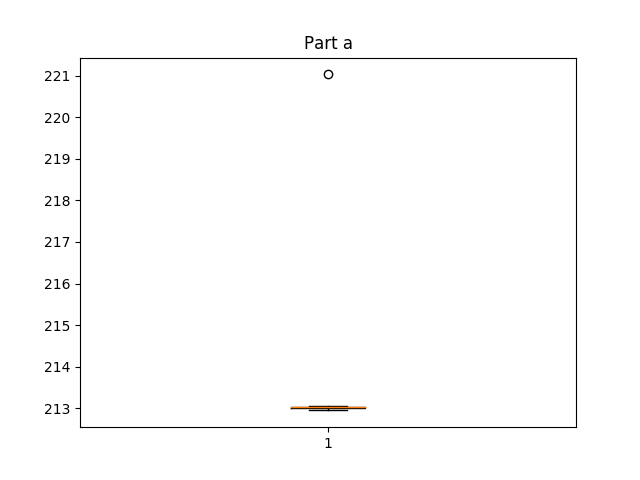
\includegraphics[width=.70\textwidth]{HW12boxplot.png}
	\end{center}
	\caption{Box plot of the given data, Showing one outliers}
   \label{fig:3}
   \end{figure}
 \item the assumptions are met
 \begin{figure}[H]
	\begin{center}
		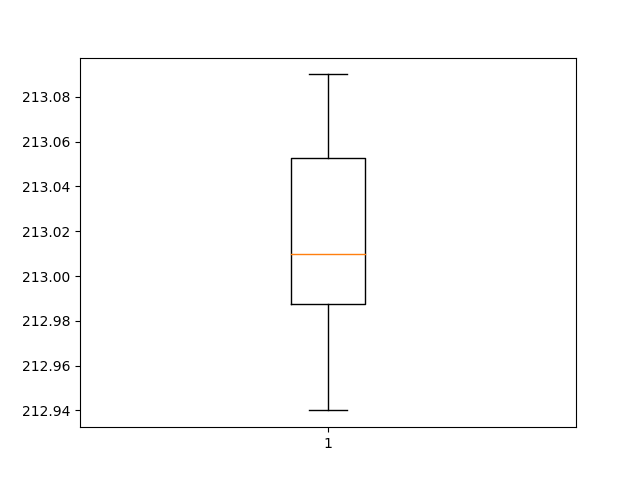
\includegraphics[width=.70\textwidth]{HW12boxplot2.png}
	\end{center}
	\caption{Box plot of the given data, Showing no outliers}
   \label{fig:3}
   \end{figure}
\item the assumptions are met
\begin{figure}[H]
	\begin{center}
		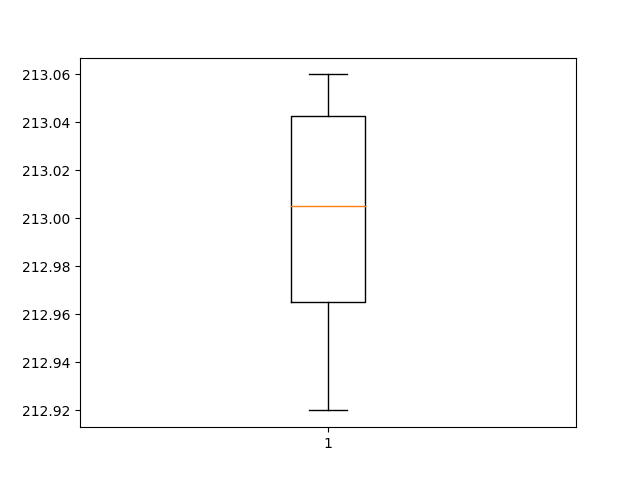
\includegraphics[width=.70\textwidth]{HW12boxplot3.png}
	\caption{Box plot of the given data, Showing no outliers}
   \label{fig:3}
	\end{center}
   \end{figure}
   \end{enumerate}   
\subsection*{6}
$$H_0:p>3.5,H_1:p\leq 3.5$$
$$S=0.084,\bar{X}=3.50667$$
 \begin{align*}
 t&=\frac{\bar{X}-\mu}{s/\sqrt{n}}\\
  &=\frac{3.50667-3.5}{.084/\sqrt{6}}\\
  &=.195\\
  &\Rightarrow\\
  &p>.05
 \end{align*}
sense p is grater than 5 $\%$ you can conclude that the mean cycle time is greater than 3.5 hours.
\end{document}